\section{Graphical-User-Interface}
To improve the ease of use of a software, it is necessary to add a Graphical-User-Interface (GUI): it brings beauty and convenience to a program since the user can navigate with the mouse and not only with the keyboard. To implement it, several choices have been made and they are explained in this part.
\subsection{Structure}
\label{sub:structure}
The main problem of the GUI is that it needs a lot of code lines to be implemented. So, the first question was: how to write the code so that it can be understandable and organized?
To answer this, the program is split into:
\begin{itemize}
	\item{\textbf{PanelCreator}} extends \textit{JFrame}. It contains all the panels and menu-bars as attributes. For each panel, there is a method \textit{createNamePanel()} and \textit{addNamePanel()}. The first one creates a new instance of the panel (and also the menu-bar if there is one associated with the panel), and adds a listener to each button. The second one sets the panel visible (and the associated menu-bar if needed) and adds it to the stack \textit{activatedPanels} (see \ref{sub:choices}).
	\item{\textbf{Launch}} contains the implementation of all the listeners which are associated to each buttons. This is only in this class that the actions of clicking on every button are define. \textbf{The main method is in this class.}
	\item Each panel corresponds to a single class which extends \textit{JPanel}. All the buttons which has to perform an action by clicking on it is put as attribute of the panel, and can be accessed in the class \textit{Launch} thanks to a getter.
	\item The classes \textbf{Error} and \textbf{Message...} represent messages which appear on the screen while clicking on a button (error message or save message for instance). So, they extends \textit{JFrame}.
\end{itemize}
Note that the creation of the panels/menu-bars, and the definition of the listeners are divided into 2 different classes.

\subsection{Choices}
\label{sub:choices}
During the implementation of the GUI, several choices have been made:
\begin{itemize}
	\item The first big choice, and maybe the most important, is not to use a single \textit{ActionListener}. Indeed, at the beginning, we wanted \textit{PanelCreator} to implement \textit{ActionListener}, and the addition of the action listener to a button who have been done by:
\lstinputlisting[firstline=1,lastline=6]{./Code/src/Code/actionListener.txt}
This means that every button has the same action listener, which leads to write in the class \textit{Launch} a lot of \textit{if} blocks like:
\lstinputlisting[firstline=1,lastline=3]{./Code/src/Code/ifBlocks.txt}
Doing so leads to a non-modular code, and difficult to understand (because it is messy). \textbf{To avoid this problem, we decided to user inner classes in the class \textit{Launch}}: each inner class implements \textit{ActionListener}.
\lstinputlisting[firstline=1,lastline=8]{./Code/src/Code/innerClasses.txt}
Doing so enables having independant listeners, and therefore the code is concerned with \textit{doing} rather than \textit{type checking}.

	\item Every user panel has the same design:
\begin{figure}[H]
	\centering
	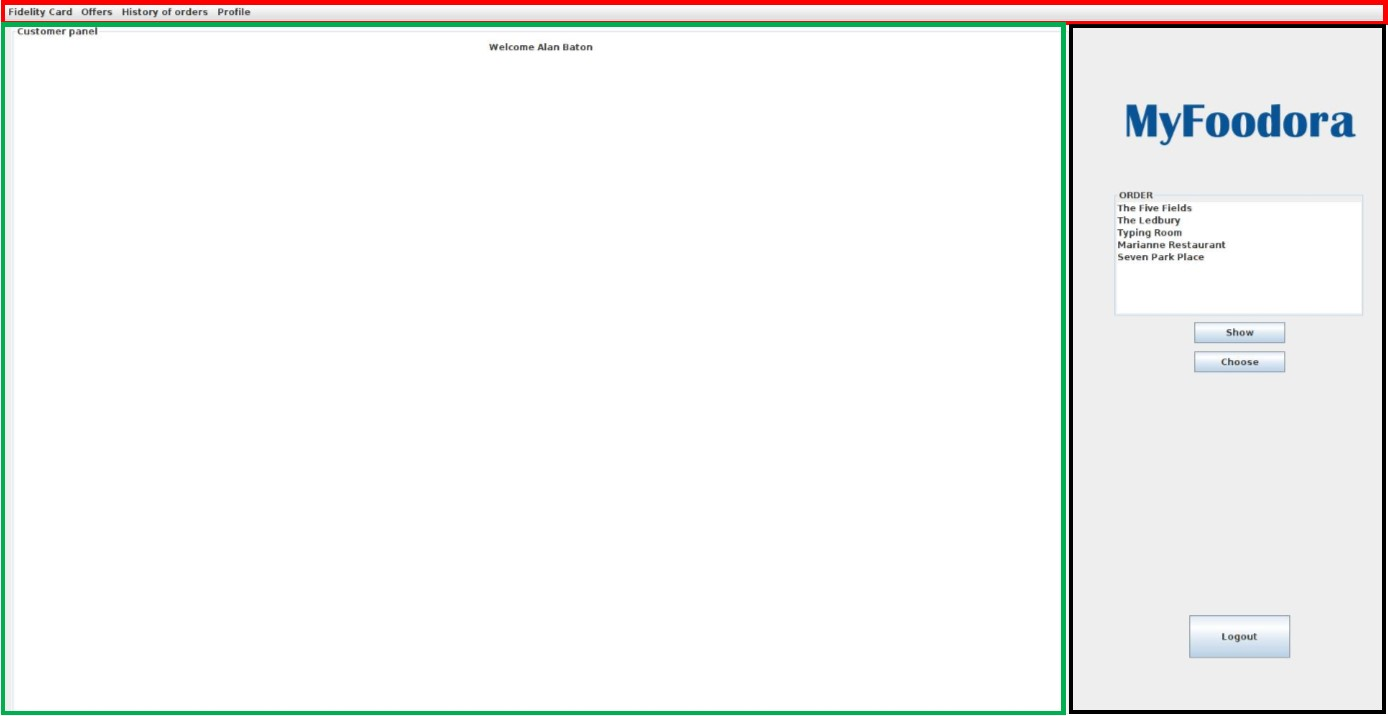
\includegraphics[width=0.8\linewidth]{./ima/designUserPanel.jpg}
	\caption{Design of a user panel}
	\label{design_of_user_panel}
\end{figure}
On the right (in black), there are the main actions the user can do, like make an order for a customer. On the top, there is a \textit{JMenuBar} (in red) containing all secondary actions like get/set the profile, get the notifications... At the center (in green), there is a big \textit{JLabel} to display the results of the actions.

	\item Almost each panel has a BACK button. \textbf{To implement the action "back", we chose to use a stack} (called \textit{activatedPanels}, attribute of \textit{PanelCreator}). Hence each time a panel is visible, it is added to the stack. When a user clicks on the BACK button, the current panel (which is the last of the stack) is removed from \textit{activatedPanels} and is set non-visible. The previous panel is then removed from the stack and becomes visible.
	
	\item To create the panels in an easy way and put the buttons where desired, \textbf{we chose to use no layout and to place and size each component with \textit{setBounds()}}. Nevertheless, at the end of the implementation of the GUI, we noticed that the compoment size depends on the resolution of the screen. As a consequence, while the panels are adapted to one pixel resolution, they can go out the screen of a different computer. To solve this problem, 2 coefficients \textit{coeffHeight} and \textit{coeffWidth} (attributes of \textit{PanelCreator}) were added. They represent the quotient of the number of pixels of the user computer divided by the number of pixels of the screen used to create the GUI.

\end{itemize}

\begin{comment}
same design for each user panel, why ?
use of menu bars, why ?
use of inner classes and not "if blocks", why ?
use of stack for back button
position/size buttons: use of pixels -> Pb computers
\end{comment}
\subsection{Scenarios}
To test the GUI, \textbf{the user has to run the main method which is in the class Launch.} Then, it is possible to register as a new user by clicking on the REGISTER button, and then login using the username and password defined previously. Otherwise, it is also possible to login directly by using the following datas:
\begin{itemize}
	\item{}Username: \textit{sparrowj}, Password: \textit{blackPearl} to login as a manager (the CEO).
	\item{}Username: \textit{batona}, Password: \textit{wer123} to login as a customer.
	\item{}Username: \textit{fiveFields}, Password: \textit{5fs} to login as a restaurant.
	\item{}Username: \textit{valmontb}, Password: \textit{1234} to login as a courier.
\end{itemize}
\label{sub:scenarios}
